\chapter{Case study and MATLAB Simulation implementation}\label{section-case}
In this chapter, an specific example\cite{hovell2017experimental} of tether satellite system is studied. In this case study, the used dynamic model and Proportional-Differentiation controller are the main analysis focuses. At the end, MATLAB simulation is also implemented.

The tether satellite system consists of two satellite and a tether. The two satellites are named as Target vehicle and Chaser vehicle which means the task of Chaser vehicle is to capture the target vehicle and to de-rotation of the system. In the real case the target vehicle can be space debris which is moving and rotation around Earth under the gravational force of the Earth. Space debris not only rotates around the Earth, in fact it will also rotate around its body center if any .De-orbiting can be achieved if the energy and angular momentum of space debris consumed.
\begin{figure}[ht]

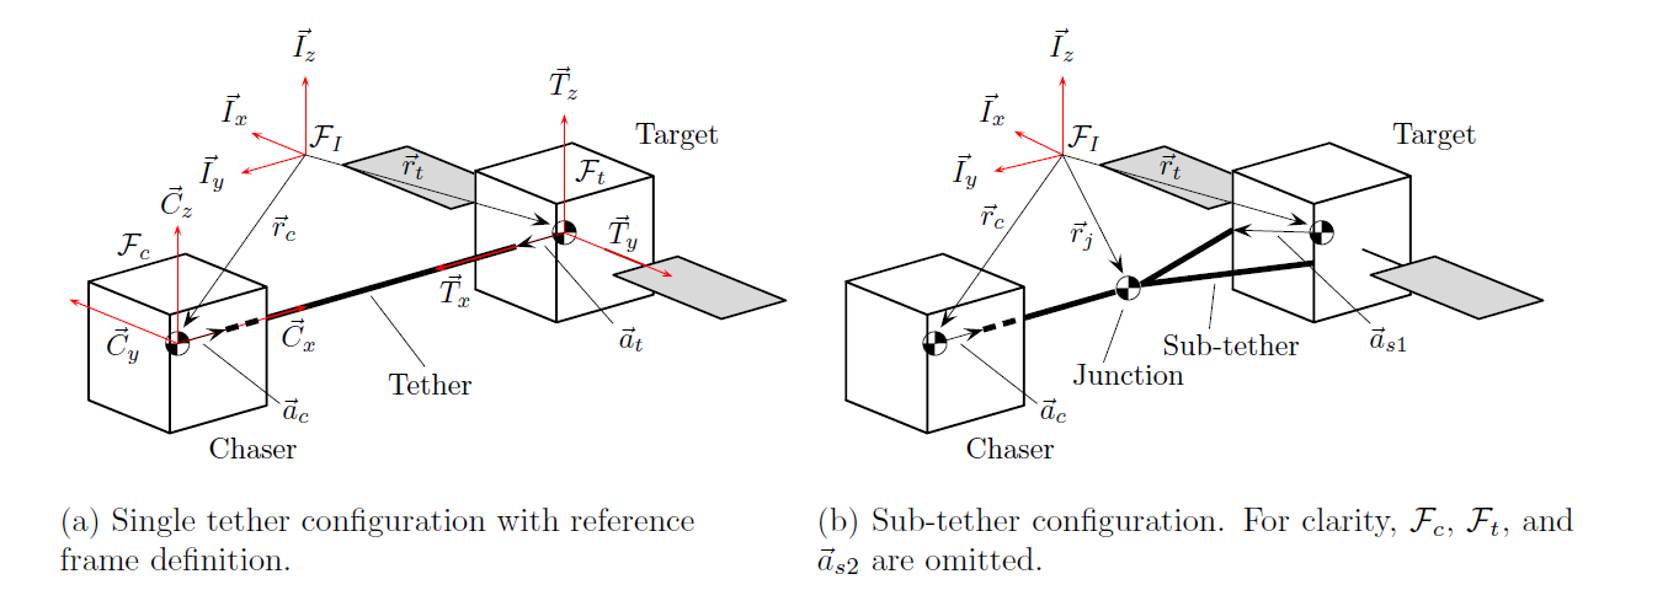
\includegraphics[width=\textwidth]{fig/simulation/ReferenceFrame}
\caption{Reference frame and vector definition for planar dynamics modeling}

\end{figure}
When we let our chaser vehicle connect with target vehicle using tether, the consumption of angular momentum becomes faster and the deorbiting gets quicker.  
So we can say that chaser vehicle plays as a role of active debris remover.

Using different kind of tether configuration, the effect of deorbiting target vehicle can be quite different.In Hovell's article, single tether confguration and sub-tether configuration are compared. The proposed sub-tether configuration can enhance the deorbiting mechanism, reducing the target tether angle and angular rate of target and finally dissipating angular momentum from the system much more quickly.  
\section{Physical Model Assumption}

\begin{itemize}

\item Massless tether, Constant end-body mass and visco-elastic tether

The tether is assumed as massless since it is much more lighter than end-body satellites.  

\item Three degree of freedom for Chaser vehicle and Target vehicle

Planar Dynamics, 
\item No external forces applied to the center of mass of the tethered satellite system

\item The Inertia matrix is constant and the 

\item Body frame of each of the end-masses is aligned with the principal axes of the end-masses


\end{itemize}

\section{}

\section{}

\section{}